\subsubsection{\stid{4.09} ADIOS} 
\paragraph{Overview} 
The Adaptable I/O Systems, ADIOS~\cite{adios2-softwarex-2020,liu2014hello}, is designed to tackle I/O and data management challenges posed  by  large-scale computational science applications running on DOE computational resources. ADIOS has  dramatically  improved  the I/O performance of Petascale  applications from a   wide range of science disciplines, thereby enabling them to accomplish their missions. The ADIOS ECP project is working on goal of transforming the ADIOS 1.x version, which has been used successfully on Petascale resources into a tool that will efficiently utilize  the underlying Exascale hardware, and create a   community I/O framework that can allow different ECP software to be easily  “plugged” into the framework. The cornerstone of this project are to 1) efficiently  address Exascale technology changes in compute, memory, and interconnect for Exascale applications; 2) develop  a  production-quality data staging method to support Exascale applications and software  technologies that require flexible in situ data reduction and management capabilities; and 3) use state  of the  art software engineering methodologies to    make it   easier for the DOE community to    use, maintain, and extend ADIOS. More precisely, our aim is to    develop and deploy a   sustainable and extensible software ecosystem. To make this into an ecosystem (rather than a point solution),this effort must result in  an  infrastructure than can be used effectively, customized, and shared among a   variety of users, Exascale applications, and hardware technologies. Technically, we are achieving  this goal  by: refactoring ADIOS  with the  goal  of improving modularity, flexibility, and extensibility by using C++; and extending, tuning, and hardening core services, such as I/O and staging that supports Exascale applications, architectures, and technologies.

\paragraph{Key  Challenges}
The core challenge of ADIOS is in its name -- adaptability.  In order to present a uniform user interface while also being able to harness the performance improvements available in the wide variety of storage and interconnect capabilities, the internal structure of the ADIOS framework must address a number of portability, functionality, and performance tuning challenges.  The internals should be constructed so that with no more than a small flag or runtime configuration a science code can move from doing I/O into a large Lustre parallel file system (with automatic calculation of file striping and number of files per directory) to utilizing burst buffer storage (with controls for delayed synchronization between the buffer and an archival store) or feeding the data directly into a concurrent application   

The challenge of supporting hardware portability and runtime performance tuning also impose a third related challenge for software engineering of the system.  In order for the code to be sustainable in the long term, while also offering guarantees of service to the end user, requires special attention to the architecture of the code base.  The consequences of trying to address these three challenges, hardware portability, runtime performance, and sustainable engineering, have driven our approach and deliverable schedule for ADIOS in ECP.

\paragraph{Solution Strategy}

The ADIOS effort has two primary thrusts:
\begin{enumerate}
	\item \textbf{Scalable I/O:} ADIOS has a data format designed for large scale parallel I/O and has data transport solutions to write/read data from/to the storage system(s) efficiently.
	\item \textbf{Scalable data staging support:}  ADIOS includes data transport solutions to work on data in transit, that is, to move data memory-to-memory, from one application stage to another without using file system I/O.
\end{enumerate}

The challenges of portability and performance apply for both of these thrusts; to a certain extent, the third challenge around software engineering emerges from the need to support these two very different categories under a single user interface.  Capitalizing on the experiences and performance expertise from our initial ADIOS platform, the ECP project wraps and extends this functionality to make it more sustainable, maintainable, and hopefully also more approachable for a wide community of users and developers.  The project approach focuses on doing deep dives with end scientist users and developers in order to make sure that the computer science development process leads to specific, verifiable results that impact the customers.


\paragraph{Recent Progress}

A new version of the Application Programming Interface unifies staging I/O and file I/O~\cite{ADIOS2-docs}, and the new, object-oriented, code framework~\cite{ADIOS2-git} supports  writing and reading files in two different file formats (ADIOS BP format and HDF5 format) and in situ with different staging implementations for various use cases. The new framework focuses on sustainable development and code reusability. The team also created the new scalable staging transport learning from the many lessons from using ADIOS for data staging and code coupling by applications in the past. As can be seen in Figure~\ref{fig:adios-example}, this past experience with methods and deep science engagements has led to demonstrations at leadership computing scale (on Titan and Summit).

\begin{figure*}[!th]
	\begin{center}
		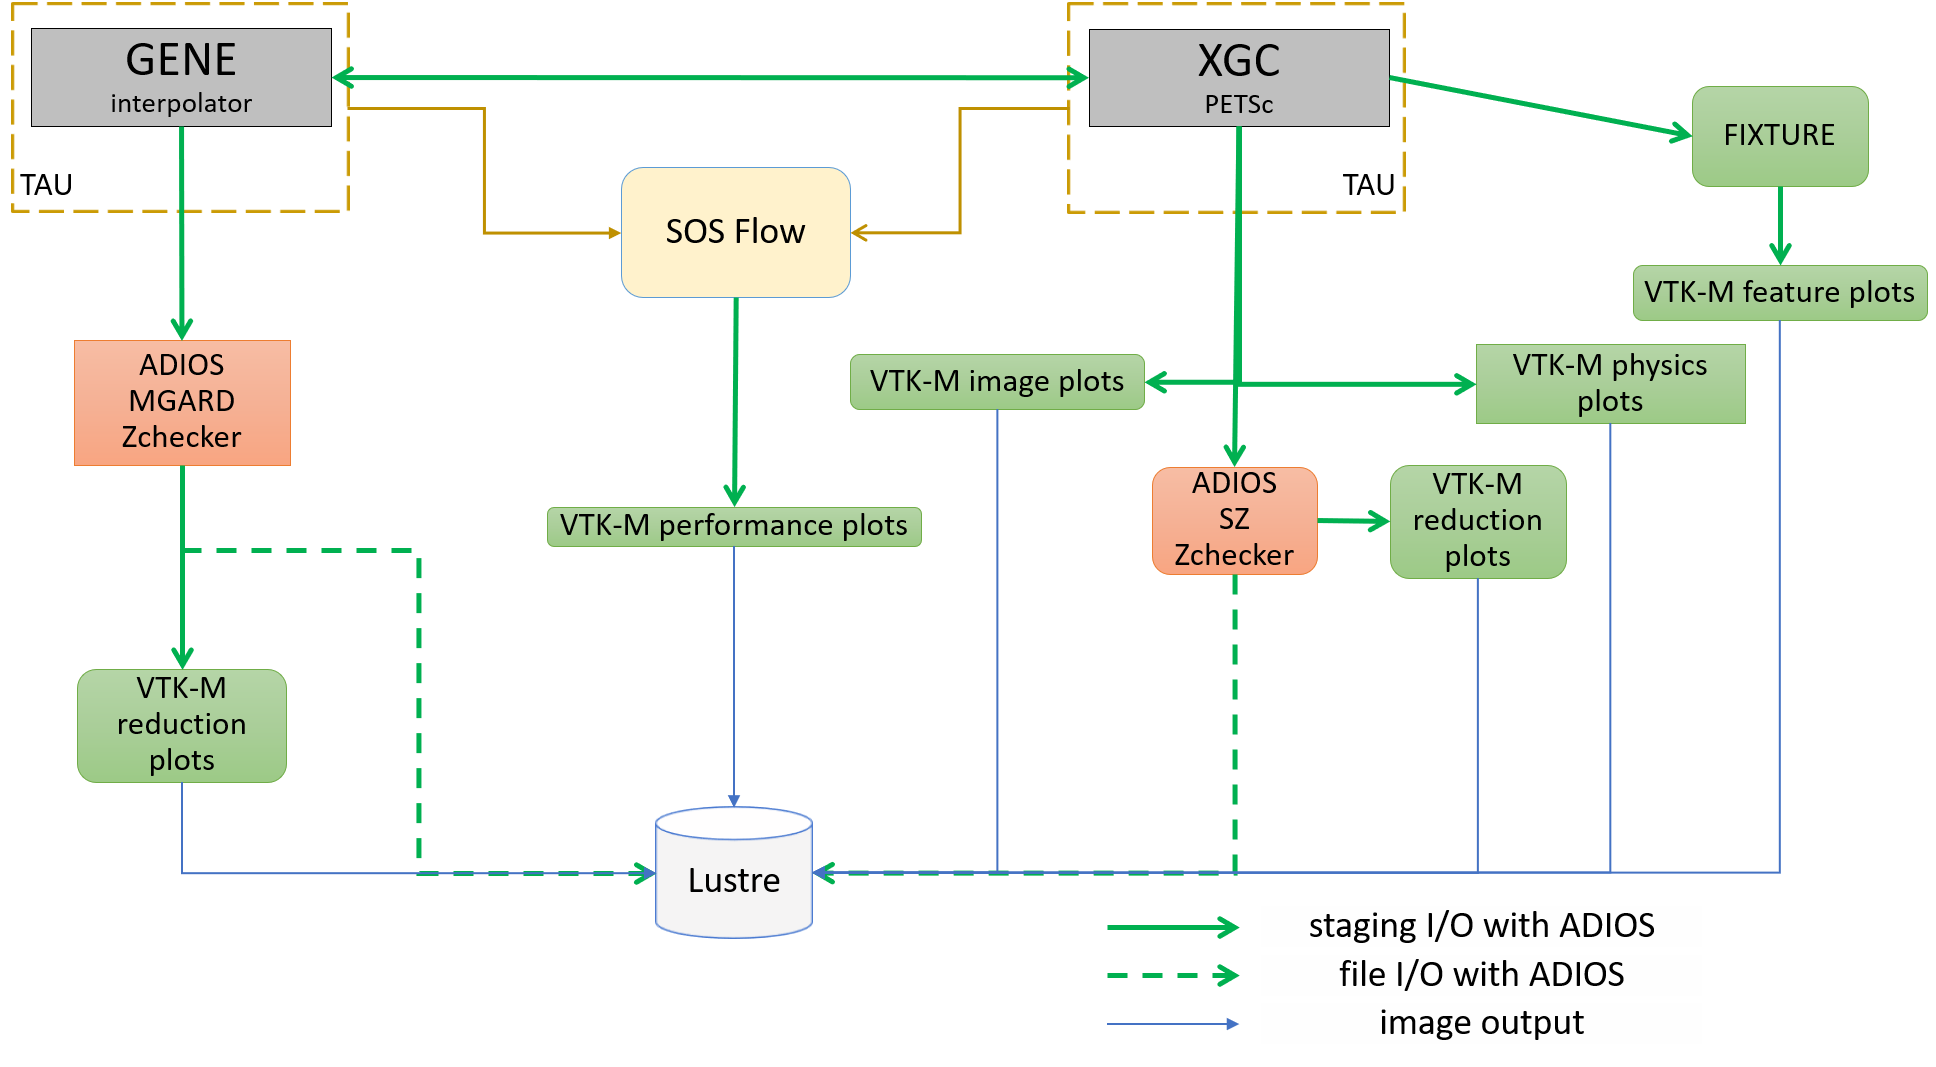
\includegraphics[width=0.75\textwidth]{projects/2.3.4-DataViz/2.3.4.09-ADIOS/ADIOS_in_ECP.png}
		\caption{An example of using ADIOS to support ECP science.  This sketch represents the demonstration at the February 2018 ECP Meeting, which featured WDM Fusion, CODAR, ADIOS, and other joint ECP activities.  Note that all of the green arrows in the figure represent data communication or storage handled by the ADIOS infrastructure.}
		\label{fig:adios-example}
	\end{center}
\end{figure*}

The new design focuses on stability and scalability so that applications can rely on it in daily production runs just as they have relied on the high performance file I/O of ADIOS. The new code base is governed with state-of-the art software development practices, including GitHub workflow of Pull-Requests with reviews, continuous integration that enforces well-tested changes to the code only, and nightly builds to catch errors on various combinations of architecture and software stack as soon as possible. Static and dynamic analysis are integrated to the GitHub workflow to catch errors before they cause trouble. Code coverage tools also help with increasing code quality. The team has access to and the code is continuously tested on DOE machines (Summit, Cori and Theta) using several ECP application codes and realistic science simulation setups (e.g. for WDMApp, E3SM-MMF and EXAALT application setups). 

For interoperability with the other main I/O library used in the ECP program, HDF5, we have added compatibility in various ways.
ADIOS has an engine to write/read HDF5 files using the original HDF5 library linked with ADIOS. A user can just change an option to switch from ADIOS-BP output to HDF5 output. On the other hand, ADIOS provides an HDF5-VOL layer, so that an HDF5 application can choose ADIOS as the underlying driver to write ADIOS-BP files from an application using HDF5. 


\paragraph{Next Steps}
In the fifth year of the project we will be focusing on some special application cases, where the internal metadata of the ADIOS data representation leads to performance problems. Notably, the E3SM-MMF and WarpX applications need a better management of ADIOS metadata and blocks of the simulation data to achieve high write and read performance at scale. We will also have effort to prepare ADIOS for the exascale machines, Frontier and Aurora. 
